\title{Comment on Jonas et. al paper}
\author{Charles Zheng and Qingyuan Zhao}
\date{\today}

\documentclass[12pt]{article} 

% packages with special commands
\usepackage{amssymb, amsmath}
\usepackage{epsfig}
\usepackage{array}
\usepackage{ifthen}
\usepackage{color}
\usepackage{fancyhdr}
\usepackage{graphicx}
\usepackage{mathtools}
\usepackage{csquotes}
\definecolor{grey}{rgb}{0.5,0.5,0.5}

\begin{document}
\maketitle

\newcommand{\tr}{\text{tr}}
\newcommand{\E}{\textbf{E}}
\newcommand{\diag}{\text{diag}}
\newcommand{\argmax}{\text{argmax}}
\newcommand{\Cov}{\text{Cov}}
\newcommand{\Var}{\text{Var}}
\newcommand{\argmin}{\text{argmin}}
\newcommand{\Vol}{\text{Vol}}
\newcommand{\comm}[1]{}

Causal inference using data from both \emph{observational}
and \emph{interventional} settings is a promising idea.  Jonas et
al. define \emph{invariant prediction sets} which can be detected
using such data, which can therefore be used to identify part of the
causal structure.  The concept of invariant prediction is quite
general, going beyond a specific modeling assumption.  However, the
bulk of the paper is devoted linear structual models; furthermore, the
specific hypothesis testing approach cannot be easily generalized
beyond the linear case.  We evaluated their approach using a dataset
which is well-known in the graphical models literature: the Sachs
et. al. protein signaling network data.  Sachs et al.  collected a
combination of observational and interventional data in order to infer
the causal structure of a network consisting of 11 proteins.  Using
their own method, Sachs et. al. reported recovering 15 of the known
directed arcs (colored black in Figure 2.)  Sachs et al. also
discovered two new putative links (not shown), and missed 3 of the
interactions which were known in the literature (dashed lines.) We
used ICP to recover part of the graph structure, taking in turn each
of the 11 variables as the response of interest and selecting the
subset of environments in which the reponse was not perturbed.  The
invariant set for each variable can be identified as the parents of
that variable in the graph.  However, for 9 of the 11 proteins, ICP
rejected the model and reported no discoveries.  For the protein PIP2,
ICP correctly identified one parent, PIP3.  For the protein PIP3, ICP
reported Mek and Jnk as part of the invariant set, but these do not
match any interactions known in the literature.

While the linear model may be overly restrictive, it is worth further
considering the general idea of combining causal and statistical
modeling assumptions in order to draw conclusions. [[for Qingyuan to write.]]

\subsection*{References}

Sachs, Karen, et al. ``Causal protein-signaling networks derived from
multiparameter single-cell data.'' Science 308.5721 (2005): 523-529.

\begin{figure}[h]
\centering
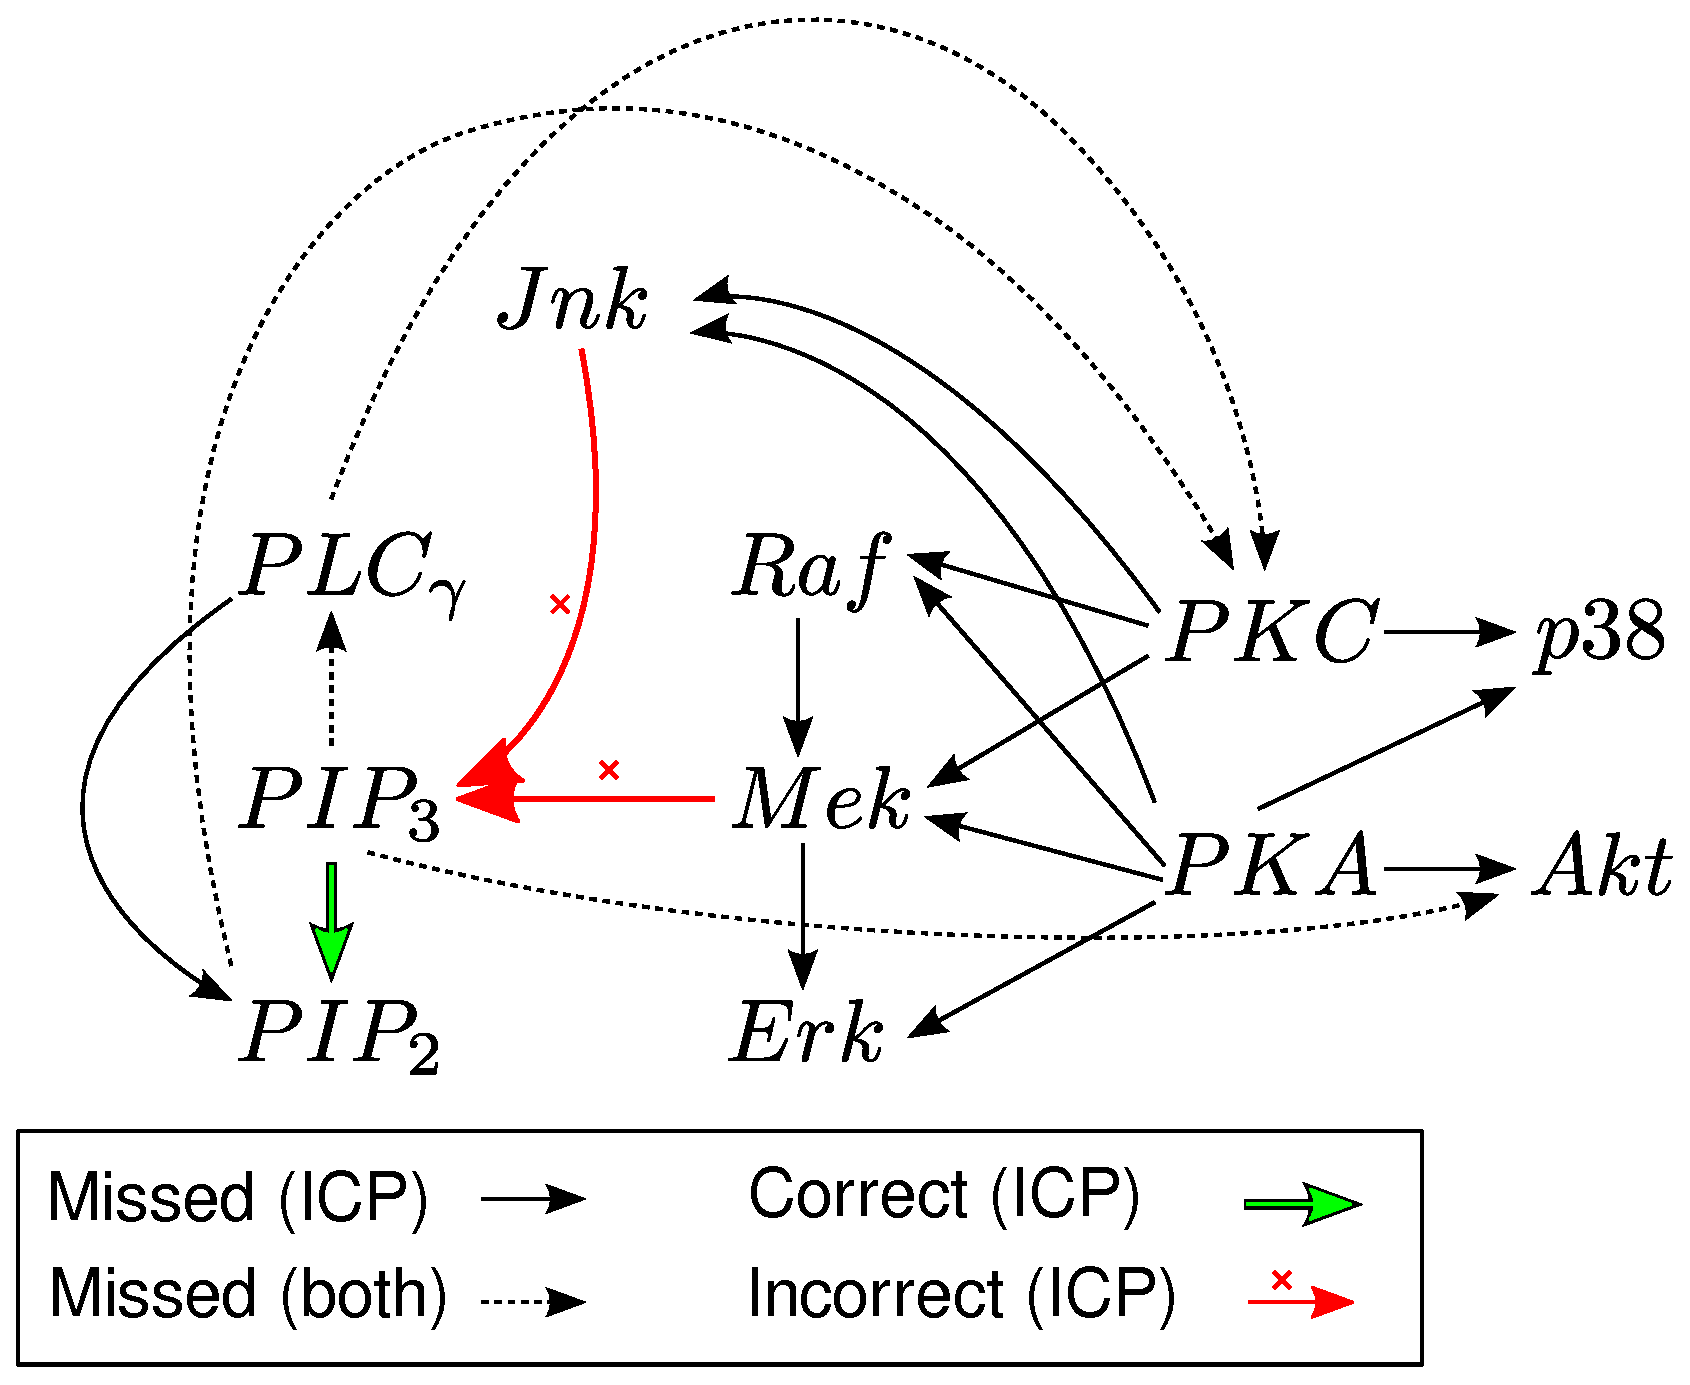
\includegraphics[scale = 0.3]{drawing2legend.eps}
\caption{Application of ICP procedure to recover protein signaling network.
ICP recovered one arrow correctly and two incorrent arrows: no other discoveries were reported.}
\end{figure}

\begin{figure}[h]
\centering
  \begin{tabular}{|c|c|}
    \hline
    \textbf{Issues} & \textbf{ICP's behavior} \\
    \hline
    Intervene on $Y$ (or a missing cause) &
    $\underset{\emptyset}{\bigcap}$ \\
    \hline
    Non-linear, non-additive, and/or heteroskedastic &
    $\underset{\emptyset}{\bigcap}$ \\
    \hline
    Not enough interventions &
    \textcolor{red}{False causal positives} \\
    \hline
    Small sample size &
    $\emptyset$ \\
    \hline
    Left out a confounder & $\underset{\emptyset}{\bigcap}$ \\
    \hline
    Left out an unconfounding predictor & okay  \\
    \hline
    Misspecified noise model$^2$ & \textcolor{red}{False positives}\\\hline
  \end{tabular}
\caption{Robustness properties of ICP procedure.  Under certain types of model misspecifiaction,
ICP will return a ``model reject'', denoted by $\cup_{\emptyset}$, rather than produce false positives.}
\end{figure}


\end{document}



